\documentclass{standalone}
\usepackage[x11names, svgnames, rgb]{xcolor}
\usepackage[utf8]{inputenc}
\usepackage{tikz}
\usetikzlibrary{snakes,arrows,shapes}
\usepackage{amsmath}
%
%

%

%

\begin{document}
\pagestyle{empty}
%
%
%

% Start of code
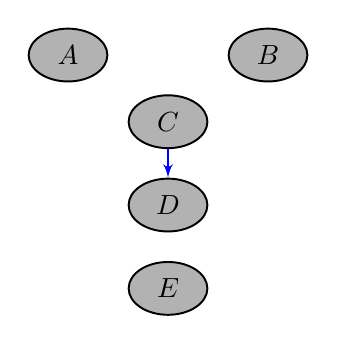
\begin{tikzpicture}[>=latex',line join=bevel,]
\pgfsetlinewidth{0.7bp}
%%
\node (A) at (27.0bp,144.0bp) [draw,fill=gray!60,ellipse, minimum width=1cm] {$A$};
  \node (C) at (63.0bp,120.0bp) [draw,fill=gray!60,ellipse, minimum width=1cm] {$C$};
  %162.0
  \node (D) at (63.0bp,90.0bp) [draw,fill=gray!60,ellipse, minimum width=1cm] {$D$};
  \node (E) at (63.0bp,60.0bp) [draw,fill=gray!60,ellipse, minimum width=1cm] {$E$};
  \node (B) at (99.0bp,144.0bp) [draw,fill=gray!60,ellipse, minimum width=1cm] {$B$};
  \draw [->, color=blue] (C) -- (D);
%
\end{tikzpicture}
% End of code

%
\end{document}
%



